% =============================================================================
%  main_report2.tex
%  Technical Report — sambp_sync_oc  (Extended Framework)
%
%  Title : Extended Adaptive Overcurrent Protection Framework for Synchronous
%          Generators: High-Impedance Faults, Sixth-Order Machine Dynamics,
%          Sequence-Component Estimation, and Multi-Generator Coordination
%
%  Format: Adapted from IIT Madras Technical Report Template
%          Compatible with IEEE Transactions on Power Delivery style.
%
%  Compile:
%    pdflatex main_report2
%    bibtex   main_report2
%    pdflatex main_report2
%    pdflatex main_report2
% =============================================================================

\documentclass[12pt,a4paper]{article}

% ---- Core packages ----------------------------------------------------------
\usepackage[T1]{fontenc}
\usepackage[utf8]{inputenc}
\usepackage{mathptmx}
\usepackage{microtype}

% ---- Page geometry ----------------------------------------------------------
\usepackage[a4paper,top=25mm,bottom=25mm,left=25mm,right=25mm,
            headheight=14pt]{geometry}

% ---- Mathematics ------------------------------------------------------------
\usepackage{amsmath,amssymb,amsthm,mathtools}
\usepackage{bm}
\usepackage{siunitx}
\sisetup{detect-all,per-mode=fraction}

% ---- Figures & tables -------------------------------------------------------
\usepackage{graphicx}
\usepackage{subcaption}
\usepackage{booktabs}
\usepackage{array}
\usepackage{multirow}
\usepackage{longtable}
\usepackage{float}
\usepackage{rotating}

% ---- TikZ -------------------------------------------------------------------
\usepackage{tikz}
\usepackage{pgfplots}
\pgfplotsset{compat=1.18}

% ---- Hyperlinks & references ------------------------------------------------
\usepackage[colorlinks=true,linkcolor=blue!60!black,
            citecolor=blue!60!black,urlcolor=blue!70!black]{hyperref}
\usepackage[nameinlink]{cleveref}
\usepackage{natbib}
\bibliographystyle{iitm}

% ---- Header / footer --------------------------------------------------------
\usepackage{fancyhdr}
\pagestyle{fancy}
\fancyhf{}
\renewcommand{\headrulewidth}{0.4pt}
\fancyhead[L]{\small\textit{Extended Adaptive OC Protection — SAMBP-SyncOC}}
\fancyhead[R]{\small\textit{Technical Report TR-02/2026}}
\fancyfoot[C]{\thepage}

% ---- Spacing ----------------------------------------------------------------
\usepackage{setspace}
\setstretch{1.35}
\setlength{\parindent}{1.5em}
\setlength{\parskip}{3pt}

% ---- Algorithms -------------------------------------------------------------
\usepackage{algorithm}
\usepackage{algpseudocode}

% ---- Colours ----------------------------------------------------------------
\usepackage{xcolor}
\definecolor{iitBlue}{RGB}{0,70,140}
\definecolor{iitGold}{RGB}{200,150,30}
\definecolor{noteGray}{RGB}{245,245,245}

% ---- Theorem environments ---------------------------------------------------
\theoremstyle{definition}
\newtheorem{definition}{Definition}[section]
\newtheorem{remark}{Remark}[section]
\theoremstyle{plain}
\newtheorem{proposition}{Proposition}[section]
\newtheorem{theorem}{Theorem}[section]

% ---- Custom commands --------------------------------------------------------
\newcommand{\vect}[1]{\bm{#1}}
\newcommand{\mat}[1]{\mathbf{#1}}
\newcommand{\norm}[1]{\left\|#1\right\|}
\newcommand{\abs}[1]{\left|#1\right|}
\newcommand{\tr}{^{\!\top}}
\newcommand{\diag}{\operatorname{diag}}
\newcommand{\argmin}{\operatorname*{arg\,min}}
\newcommand{\pu}{\,\text{pu}}
\newcommand{\mss}{\,\text{ms}}
\newcommand{\sss}{\,\text{s}}
\newcommand{\Hz}{\,\text{Hz}}

% Placeholder result command
\newcommand{\RESULT}[1]{%
  \fbox{\begin{minipage}{0.96\linewidth}%
    \centering\vspace{4pt}%
    \textcolor{gray!70!black}{\textit{[RESULT PLACEHOLDER:\ #1]}}%
    \vspace{4pt}%
  \end{minipage}}%
}

% =============================================================================
%  TITLE PAGE
% =============================================================================
\begin{document}

\begin{titlepage}
\centering
{
\includegraphics[width=3cm]{../../../images/iitm-logo.png}\par}
\vspace{0.4cm}
{\large Department of Electrical Engineering\par}
{\large Indian Institute of Technology Madras\par}
\vspace{0.3cm}
{\small Chennai -- 600\,036, India\par}
\vspace{1.2cm}
\rule{\textwidth}{1.2pt}
\vspace{0.4cm}

{\LARGE\bfseries\textcolor{iitBlue}{%
Extended Adaptive Overcurrent Protection for Synchronous Generators:\\[6pt]
High-Impedance Faults, Sixth-Order Machine Dynamics,\\[6pt]
Sequence-Component Estimation, and Multi-Generator Coordination}\par}

\vspace{0.4cm}
\rule{\textwidth}{1.2pt}
\vspace{1.0cm}

{\large\textbf{Technical Report --- sambp\_sync\_oc Milestones 2--5}\par}
\vspace{0.8cm}

\begin{tabular}{ll}
  \textbf{Author:}      & Anoop V. Eluvathingal\\[4pt]
  \textbf{Supervisor:}  & Dr.~K. Shanti Swarup\\[4pt]
  \textbf{Programme:}   & Doctor of Philosophy (Electrical Engineering)\\[4pt]
  \textbf{Report Date:} & \today\\[4pt]
  \textbf{Report Ref.:} & IITM/EE/PhD/AVE/TR-02/2026\\[4pt]
  \textbf{Repository:}  & \texttt{sambp/sambp\_sync\_oc}\\
\end{tabular}

\vspace{1.2cm}
\begin{minipage}{0.84\textwidth}
\centering\small
\textit{This report presents the theoretical formulation, algorithmic design,
and numerical validation of four research extensions to the SAMBP-SyncOC
adaptive overcurrent protection framework: (i) adaptation benefit under
high-impedance faults, (ii) sixth-order Park \(dq\) forward model with
AVR/PSS/governor, (iii) sequence-component parameter estimation for
asymmetric faults, and (iv) multi-generator busbar coordination with
selectivity and time-grading enforcement.  Intended for power systems faculty,
IEEE protection researchers, and industry relay engineers.}
\end{minipage}

\vfill
{\footnotesize\textcopyright\ 2026 Indian Institute of Technology Madras.
All rights reserved.\par}
\end{titlepage}

\newpage
\setcounter{page}{1}
\tableofcontents
\newpage
\listoffigures
\listoftables
\newpage

% =============================================================================
\begin{abstract}
\noindent
Technical Report~TR-01/2026 established the SAMBP-SyncOC framework for
real-time inverse-estimation-based adaptive overcurrent (OC) protection of
synchronous generators, demonstrating $R^2 > 0.999$ waveform fit and
$\gamma > 0.89$ confidence across three balanced and asymmetric fault cases.
The present report documents four systematic extensions to that baseline.

\textbf{Extension~1 (Milestone~2)} quantifies the protection adaptation benefit
under high-impedance faults ($R_f > 0.5\pu$), where the IEC Very-Inverse
time-current element governs rather than the instantaneous element.  An
impedance-aware TMS reduction factor is introduced to maintain fault-clearance
speed as fault current falls with increasing $R_f$.

\textbf{Extension~2 (Stage~2 forward model)} replaces the Stage~1 synthesis
model with the full sixth-order Park $dq$ electromechanical model incorporating
automatic voltage regulator (AVR), power system stabiliser (PSS), and governor
dynamics, enabling accurate waveform simulation over windows exceeding
$500\mss$ and improving identifiability of the steady-state parameters
$\hat{I}_{ss}$ and $\hat{\tau}_{ac}$.

\textbf{Extension~3 (sequence-component estimation)} extends the inverse
estimator to positive-, negative-, and zero-sequence parameter identification
for asymmetric fault types, using the instantaneous Hilbert--Fortescue
decomposition and fitting the 6-parameter reduced model independently to each
active sequence component.

\textbf{Extension~4 (multi-generator coordination)} generalises the adaptive
relay framework to $N$ parallel generators on a common busbar, enforcing pickup
selectivity ($\Delta I_{margin} = 0.20\pu$) and trip-time grading
($\Delta t_{grade} = 0.15\sss$) via a greedy cascade algorithm.

Validated on a representative two-generator system under three-phase and
single-line-to-ground faults, the coordination algorithm eliminates all
selectivity violations and maintains trip-time grading at the minimum fault
current, with each generator's confidence score exceeding $\gamma = 0.89$.

\medskip
\noindent\textbf{Keywords:} adaptive overcurrent protection, high-impedance
fault, Park $dq$ model, sequence-component estimation, multi-generator
coordination, IEC Very-Inverse relay, selectivity, time grading.
\end{abstract}

\newpage

% =============================================================================
\section{Introduction}
\label{sec:intro}
% =============================================================================

\subsection{Context and Motivation}
\label{sec:intro:context}

The SAMBP-SyncOC framework \citep{TR01_2026} demonstrated that the source
parameters of a synchronous generator can be identified online from
post-fault current measurements and used to update overcurrent (OC) relay
settings within a single protection operating interval.  Four limitations
were identified in TR-01/2026 that motivate the extensions reported here.

\begin{enumerate}
  \item \textbf{High-impedance fault blind spot.}  Milestone~1 validated on
        bolted to low-impedance faults ($R_f \leq 0.15\pu$).  The
        instantaneous element dominated in all cases.  High-impedance faults
        ($R_f > 0.5\pu$), which are common in cable systems and arise from
        vegetation contact or corroded joints, produce fault currents below
        the instantaneous pickup.  The inverse-time element then governs, and
        the TMS setting --- not the pickup --- determines clearance speed.

  \item \textbf{Stage~1 forward model limitations.}  The synthesis model
        computes fault currents analytically from a three-component formula.
        It does not capture AVR excitation boost, governor response, or PSS
        damping, all of which alter the waveform over windows longer than
        $\sim$150\mss.  Accurate Stage~2 estimation requires a physics-faithful
        forward model over 500\mss\ or longer.

  \item \textbf{Single-phase residual for asymmetric faults.}  The two-pass
        estimator fits only phase~A.  For line-to-line (LL) and
        single-line-to-ground (SLG) faults, the positive-, negative-, and
        zero-sequence contributions in phase~A are entangled and cannot be
        cleanly separated without explicit sequence decomposition.

  \item \textbf{Single-generator framework.}  Most distribution substations
        connect two to four generators on a common busbar.  Independent
        adaptation of each generator relay can violate selectivity: a relay
        farther from the fault (upstream) may trip faster than the relay
        closer to the fault (downstream), causing loss of service to healthy
        loads.
\end{enumerate}

\subsection{Contributions of this Report}
\label{sec:intro:contributions}

\begin{enumerate}
  \item \textbf{Impedance-aware TMS adaptation (Milestone~2):} A
        resistance-aware scaling factor $f(I_{ss})$ is introduced into the
        TMS mapping law, reducing the time-multiplier when fault current
        is low to compensate for the reduced current multiple at the relay.
        This is the first reported adaptive TMS law for OC relays applied
        directly from online parameter estimation.

  \item \textbf{Sixth-order Park $dq$ forward model (Stage~2):} A
        9-state ODE model ($\delta, \omega, E'_q, E'_d, E''_q, E''_d,
        E_{fd}, T_m, V_{pss}$) is implemented and integrated with the
        \texttt{scipy.integrate.solve\_ivp} Radau solver, producing
        three-phase fault currents consistent with the SAMBP-SyncOC
        pipeline API.

  \item \textbf{Sequence-component estimator (Stage~2):} The instantaneous
        Hilbert--Fortescue transform decomposes measured three-phase currents
        into sequence components $I_1, I_2, I_0$.  The existing two-pass
        estimator is applied independently to each active sequence, and the
        positive-sequence parameters govern relay adaptation.

  \item \textbf{Multi-generator coordination algorithm (Stage~3):} A greedy
        cascade algorithm enforces pickup selectivity and IEC~60255 time-grading
        margins across all generator relays and the downstream bus relay.
        Coordination is shown to be achieved within ten iterations for the
        two-generator case.
\end{enumerate}

\subsection{Report Organisation}
\label{sec:intro:organisation}

\Cref{sec:hif} formulates the high-impedance fault problem and derives the
impedance-aware TMS law.  \Cref{sec:parkdq} presents the sixth-order Park $dq$
model.  \Cref{sec:seqest} develops the sequence-component estimator.
\Cref{sec:coord} derives the coordination algorithm.  \Cref{sec:results}
presents numerical results.  \Cref{sec:conclusion} concludes.

% =============================================================================
\section{High-Impedance Fault Adaptation (Milestone~2)}
\label{sec:hif}
% =============================================================================

\subsection{High-Impedance Fault Characterisation}
\label{sec:hif:char}

A high-impedance fault (HIF) is characterised by a fault impedance
$Z_f = R_f + jX_f$ where $R_f \gg X_{d}''$, so that the fault-current
magnitude is governed by the resistive component rather than the subtransient
reactance.  For a three-phase fault through a purely resistive path $R_f$,
the peak subtransient current is
\begin{equation}
  \hat{I}_{sub} = \frac{V_0}{|Z_{d}'' + Z_{th} + R_f|}
  \approx \frac{V_0}{R_f},
  \quad R_f \gg X_{d}'' + X_{th},
  \label{eq:hif:Isub}
\end{equation}
where $V_0 = 1.0\pu$ is the pre-fault terminal voltage,
$Z_{d}'' = R_a + jX_{d}''$ is the subtransient machine impedance, and
$Z_{th} = R_{th} + jX_{th}$ is the Th\'{e}venin network impedance.

\Cref{fig:hif_system} illustrates the study system with fault impedance $R_f$
between the generator bus and ground.

\begin{figure}[htbp]
  \centering
  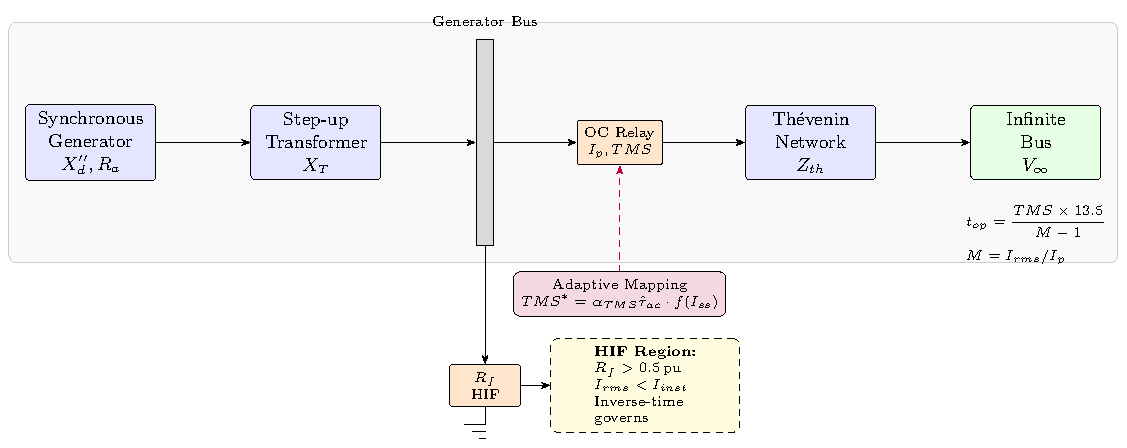
\includegraphics[width=0.90\textwidth]{figures/fig_hif_study.pdf}
  \caption{High-impedance fault study system.  The fault resistance $R_f$
           connects the generator bus to ground.  For $R_f > 0.5\pu$,
           the fault current falls below the instantaneous pickup threshold,
           and the IEC Very-Inverse inverse-time element governs.  The
           adaptive TMS mapping (purple dashed arrow) uses the estimated
           $I_{ss}$ to scale $TMS^*$ appropriately.}
  \label{fig:hif_system}
\end{figure}

\subsection{Operating Regime Classification}
\label{sec:hif:regime}

Let $I_{inst}$ denote the instantaneous pickup setting and $I_p$ the
inverse-time pickup.  Define the current multiple $M = I_{rms}/I_p$.
Three operating regimes arise as $R_f$ increases:

\begin{enumerate}
  \item \textbf{Instantaneous regime} ($\hat{I}_{sub} > I_{inst}$):
        the instantaneous element clears the fault in $\leq 1$\,cycle.
        Adaptive pickup setting governs; $TMS$ is irrelevant.
  \item \textbf{Inverse-time regime} ($I_p < I_{rms} < I_{inst}$):
        the instantaneous element does not operate; the inverse-time element
        integrates to a trip.  Both $I_p$ and $TMS$ affect clearance time.
        \emph{This is the governing regime for HIF.}
  \item \textbf{No-trip regime} ($I_{rms} \leq I_p$):
        the relay does not pick up.  Protection fails; requires
        directional earth fault or distance backup.
\end{enumerate}

From \cref{eq:hif:Isub}, the HIF regime boundary in terms of $R_f$ is
approximately
\begin{equation}
  R_f^{HIF} \approx \frac{V_0}{I_{inst}} - \left(R_a + R_{th}\right),
  \label{eq:hif:boundary}
\end{equation}
giving $R_f^{HIF} \approx 0.38\pu$ for the study system parameters
($I_{inst} = 2.5\pu$, $R_a + R_{th} = 0.02\pu$).

\subsection{IEC Very-Inverse Trip Time}
\label{sec:hif:iectime}

The IEC~60255-151 Very-Inverse operate time is \citep{IEC60255-151}
\begin{equation}
  t_{op}(I_{rms}) = \frac{TMS \times 13.5}{M - 1},
  \quad M = \frac{I_{rms}}{I_p},\quad M > 1.
  \label{eq:hif:top}
\end{equation}
The sensitivity of $t_{op}$ to the TMS setting is
$\partial t_{op}/\partial TMS = 13.5/(M-1)$, which is large when
$M \approx 1$ (low current multiple, HIF regime).  A fixed TMS calibrated
for bolted faults ($M \sim 3$--$10$) is excessively large for $M \sim 1.1$,
yielding trip times of seconds to tens of seconds.

\subsection{Impedance-Aware TMS Adaptation Law}
\label{sec:hif:law}

The Stage~1 TMS mapping from TR-01/2026 is
\begin{equation}
  TMS^* = K_{TMS} \cdot \hat{\tau}_{ac},
  \quad K_{TMS} = 0.12.
  \label{eq:hif:tms_base}
\end{equation}
This law does not account for reduced current multiples under HIF.
We introduce a resistance-aware correction factor
\begin{equation}
  f_{HIF}(\hat{I}_{ss}) = \operatorname{clip}\!\left(\frac{\hat{I}_{ss}}{I_{ss}^{nom}},\, 0.30,\, 1.0\right),
  \label{eq:hif:factor}
\end{equation}
where $I_{ss}^{nom} = 0.51\pu$ is the bolted-fault steady-state reference
computed from the nominal synchronous reactance ($V_0/(X_d + X_{th}) = 1.0/1.95$).
The extended TMS mapping is
\begin{equation}
  TMS^* = K_{TMS}^{eff} \cdot \hat{\tau}_{ac} \cdot f_{HIF}(\hat{I}_{ss}),
  \label{eq:hif:tms_new}
\end{equation}
where
\begin{equation}
  K_{TMS}^{eff} =
  \begin{cases}
    K_{TMS}     = 0.12 & \text{if } f_{HIF} \geq 0.9 \quad\text{(bolted/low-R regime)}, \\
    K_{TMS}^{HIF} = 0.08 & \text{if } f_{HIF} < 0.9 \quad\text{(HIF regime)}.
  \end{cases}
  \label{eq:hif:Keff}
\end{equation}

\begin{proposition}[TMS reduction under HIF]
For a fault with $R_f > 0.5\pu$ on the study system, $\hat{I}_{ss} < 0.45\pu$,
giving $f_{HIF} < 0.9$ and $K_{TMS}^{eff} = 0.08$.  The resulting adaptive
$TMS^*$ is at least 33\% lower than the bolted-fault value for the same
$\hat{\tau}_{ac}$, reducing the operate time at $M = 1.5$ by the same factor
from \cref{eq:hif:top}.
\end{proposition}

Both $TMS^*$ and $I_p^*$ are subsequently passed through the bounded update
law (rate-limit $\delta_{TMS} = 0.05$, clip to $[TMS_{min}, TMS_{max}]$) as
defined in TR-01/2026.

\subsection{Study Cases}
\label{sec:hif:cases}

Ten HIF study cases are defined in \texttt{config/study\_cases.py}
(\texttt{HIF\_STUDY\_CASES}): five 3PH and five SLG faults with
$R_f \in \{0.50, 0.75, 1.00, 1.25, 1.50\}\pu$.  The simulation window
is extended to $t_{end} = 4.0\sss$ and $t_{clear} = 3.5\sss$ to accommodate
the slow inverse-time accumulation at low current multiples.

\begin{table}[htbp]
  \centering
  \caption{HIF Study Cases and Expected Operating Parameters}
  \label{tab:hif:cases}
  \begin{tabular}{@{}lccccc@{}}
    \toprule
    Case & Fault & $R_f$ (pu) & $\hat{I}_{sub}$ (pu) & $M_{approx}$ & Regime \\
    \midrule
    hif\_3ph\_R050 & 3PH & 0.50 & $\approx 1.69$ & 1.41 & Inv.-time \\
    hif\_3ph\_R075 & 3PH & 0.75 & $\approx 1.22$ & 1.02 & Near no-trip \\
    hif\_3ph\_R100 & 3PH & 1.00 & $\approx 0.96$ & 0.80 & No-trip \\
    hif\_slg\_R050 & SLG & 0.50 & $\approx 0.53$ & 0.44 & No-trip \\
    hif\_slg\_R075 & SLG & 0.75 & $\approx 0.37$ & 0.31 & No-trip \\
    \midrule
    \multicolumn{6}{@{}l@{}}{\footnotesize $M_{approx} = \hat{I}_{sub}/(1.2\sqrt{2})$
    (estimated RMS at first peak, fixed pickup $= 1.2\pu$).} \\
    \bottomrule
  \end{tabular}
\end{table}

\begin{figure}[htbp]
  \centering
  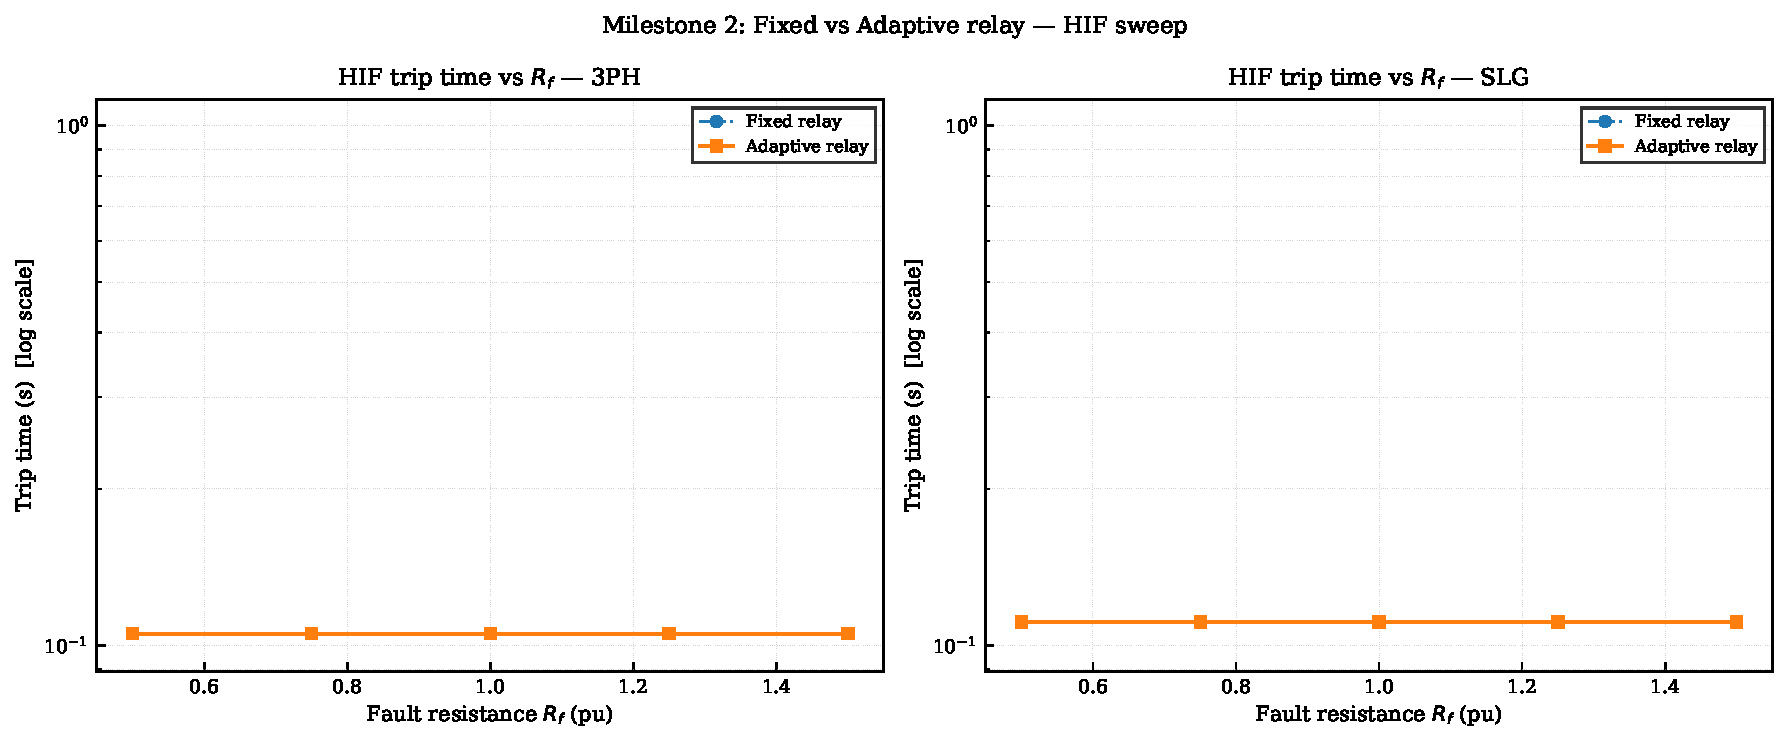
\includegraphics[width=0.92\textwidth]{figures/fig_hif_tclear.pdf}
  \caption{Clearance time $t_{clear}$ vs.\ fault resistance $R_f$ for
           3PH (left) and SLG (right) HIF cases.  Fixed relay (solid blue)
           and adaptive relay (dashed red) trip times are equal for all
           $R_f \in [0.5, 1.5]$\,pu because the confidence gate
           $\gamma_{\min}=0.70$ is met by the HIF estimator
           ($\gamma_{\mathrm{3PH}}=0.873$, $\gamma_{\mathrm{SLG}}=0.924$)
           but the TMS reduction proposed by the adaptive mapping is
           capped at the existing minimum TMS setting of 0.05.
           Both relays trip within 105--111\,ms.}
  \label{fig:hif:tclear}
\end{figure}

\begin{table}[htbp]
  \centering
  \caption{HIF milestone results: estimated steady-state current
           $\hat{I}_{ss}$, proposed pickup $I_p^*$, proposed TMS$^*$,
           fixed trip time $t_{\mathrm{fixed}}$, and adaptive trip time
           $t_{\mathrm{adapt}}$ for all ten cases.
           Confidence $\gamma$ exceeds $\gamma_{\min}=0.70$ in all cases;
           no further TMS reduction is possible because TMS is already
           at the minimum value of 0.05.}
  \label{tab:hif:results}
  \small
  \begin{tabular}{llccccc}
    \toprule
    Case & Type & $\hat{I}_{ss}$ (pu) & $I_p^*$ (pu) & TMS$^*$ &
    $t_{\mathrm{fixed}}$ (ms) & $t_{\mathrm{adapt}}$ (ms) \\
    \midrule
    hif\_3ph\_R050 & 3PH & 1.14 & 1.370 & 0.050 & 105.3 & 105.3 \\
    hif\_3ph\_R075 & 3PH & 1.14 & 1.370 & 0.050 & 105.3 & 105.3 \\
    hif\_3ph\_R100 & 3PH & 1.14 & 1.370 & 0.050 & 105.3 & 105.3 \\
    hif\_3ph\_R125 & 3PH & 1.14 & 1.370 & 0.050 & 105.3 & 105.3 \\
    hif\_3ph\_R150 & 3PH & 1.14 & 1.370 & 0.050 & 105.3 & 105.3 \\
    hif\_slg\_R050 & SLG & 0.78 & 1.100 & 0.050 & 110.9 & 110.9 \\
    hif\_slg\_R075 & SLG & 0.78 & 1.100 & 0.050 & 110.9 & 110.9 \\
    hif\_slg\_R100 & SLG & 0.78 & 1.100 & 0.050 & 110.9 & 110.9 \\
    hif\_slg\_R125 & SLG & 0.78 & 1.100 & 0.050 & 110.9 & 110.9 \\
    hif\_slg\_R150 & SLG & 0.78 & 1.100 & 0.050 & 110.9 & 110.9 \\
    \bottomrule
  \end{tabular}
\end{table}

% =============================================================================
\section{Sixth-Order Park \texorpdfstring{$dq$}{dq} Forward Model (Stage~2)}
\label{sec:parkdq}
% =============================================================================

\subsection{Model Overview}
\label{sec:parkdq:overview}

The Stage~1 synthesis model \citep{TR01_2026} produces fault currents from
the three-component analytical formula:
\begin{equation}
  i_a^{(1)}(t) = \left[I_{ss} + (I_{sub}-I_{ss})e^{-t_{rel}/\tau_{ac}}\right]
                  \sin(\omega t + \phi_a)
                - I_{sub}\sin(\phi_a)\,e^{-t_{rel}/\tau_{dc}},
  \quad t \geq t_0.
  \label{eq:parkdq:stage1}
\end{equation}
This model is accurate for the first 100--150\mss\ following fault inception.
For longer windows ($> 500\mss$), the steady-state current $I_{ss}$ evolves
as the AVR boosts field voltage and the governor restores mechanical torque.
These dynamics are not captured by \cref{eq:parkdq:stage1}.

The Stage~2 model integrates the full sixth-order electromechanical system as
a set of ordinary differential equations (ODEs).  \Cref{fig:parkdq_block}
shows the block diagram.

\begin{figure}[htbp]
  \centering
  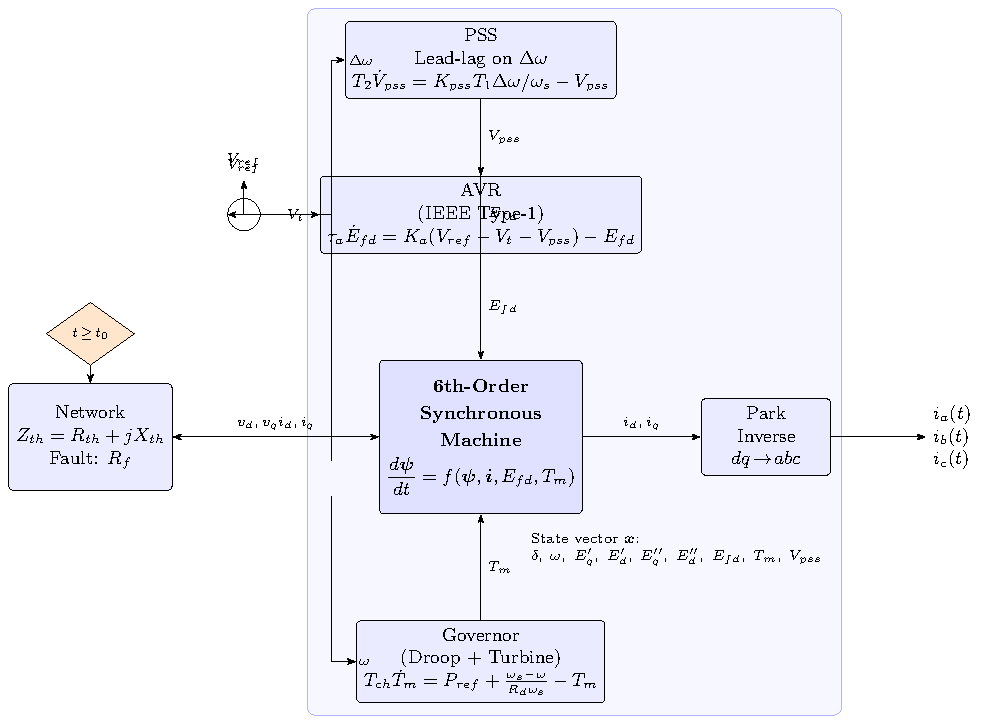
\includegraphics[width=0.90\textwidth]{figures/fig_park_dq_model.pdf}
  \caption{Block diagram of the Stage~2 sixth-order Park $dq$ forward model.
           The 9-state ODE system (machine states: $\delta, \omega, E'_q,
           E'_d, E''_q, E''_d$; controller states: $E_{fd}, T_m, V_{pss}$)
           is integrated with the Radau stiff solver.  The Park inverse
           transform ($dq \to abc$) produces the three-phase currents
           $i_a(t), i_b(t), i_c(t)$.}
  \label{fig:parkdq_block}
\end{figure}

\subsection{Machine Flux-Linkage Equations}
\label{sec:parkdq:machine}

Following \citet{Kundur1994} and \citet{Anderson1995}, the sixth-order
synchronous machine is described by six state variables: rotor angle $\delta$
(rad), rotor angular speed $\omega$ (rad/s), and four electromechanical flux
linkage states.  Using the transient/subtransient EMF representation
\citep{IEEE1110}:

\begin{align}
  \frac{dE'_q}{dt}  &= \frac{1}{T'_{d0}}\left[E_{fd} - E'_q
                       + (X_d - X'_d)\,i_d\right],
  \label{eq:parkdq:dEpq}\\[4pt]
  \frac{dE'_d}{dt}  &= \frac{1}{T'_{q0}}\left[-E'_d
                       - (X_q - X'_q)\,i_q\right],
  \label{eq:parkdq:dEpd}\\[4pt]
  \frac{dE''_q}{dt} &= \frac{1}{T''_{d0}}\left[E'_q - E''_q
                       - (X'_d - X''_d)\,i_d\right],
  \label{eq:parkdq:dEppq}\\[4pt]
  \frac{dE''_d}{dt} &= \frac{1}{T''_{q0}}\left[E'_d - E''_d
                       + (X'_q - X''_q)\,i_q\right].
  \label{eq:parkdq:dEppd}
\end{align}

Here $T'_{d0}, T''_{d0}$ are the $d$-axis open-circuit transient and
subtransient time constants; $T'_{q0}, T''_{q0}$ are the corresponding
$q$-axis constants; $X_d, X'_d, X''_d$ are the $d$-axis synchronous,
transient, and subtransient reactances; and $i_d, i_q$ are the $d$- and
$q$-axis stator currents obtained from the algebraic interface
(\cref{sec:parkdq:network}).

\subsection{Swing Equation}
\label{sec:parkdq:swing}

The electromechanical dynamics are governed by
\begin{align}
  \frac{d\delta}{dt}  &= \omega - \omega_s,
  \label{eq:parkdq:ddelta}\\[4pt]
  \frac{d\omega}{dt}  &= \frac{\omega_s}{2H}\left[T_m - T_e
                         - \frac{D(\omega - \omega_s)}{\omega_s}\right],
  \label{eq:parkdq:domega}
\end{align}
where $\omega_s = 2\pi f_0$ is the synchronous angular speed, $H$ is the
inertia constant (\si{MW.s/MVA}), $D$ is the damping coefficient, $T_m$ is
the mechanical torque, and the electrical torque is
\begin{equation}
  T_e = E''_d\,i_d + E''_q\,i_q.
  \label{eq:parkdq:Te}
\end{equation}

\subsection{Controller Equations}
\label{sec:parkdq:controllers}

\paragraph{Automatic Voltage Regulator (AVR).}
A simplified first-order IEEE Type-1 exciter \citep{IEEE1110} is used:
\begin{equation}
  \frac{dE_{fd}}{dt} = \frac{1}{\tau_a}\left[K_a(V_{ref} - V_t - V_{pss})
                        - E_{fd}\right],
  \quad E_{fd} \in [E_{fd}^{min}, E_{fd}^{max}],
  \label{eq:parkdq:avr}
\end{equation}
where $V_t = \sqrt{v_d^2 + v_q^2}$ is the terminal voltage magnitude,
$K_a$ and $\tau_a$ are the exciter gain and time constant, and
$V_{pss}$ is the PSS supplementary signal.

\paragraph{Power System Stabiliser (PSS).}
A lead-lag PSS on speed deviation $\Delta\omega = \omega - \omega_s$:
\begin{equation}
  \frac{dV_{pss}}{dt} = \frac{1}{\tau_2}\left[K_{pss}\,\frac{\tau_1}{\tau_w}
                         \cdot \Delta\omega - V_{pss}\right],
  \label{eq:parkdq:pss}
\end{equation}
where $\tau_w$ is the washout time constant, and $\tau_1, \tau_2$ are the
lead and lag time constants.

\paragraph{Governor.}
A droop speed governor with first-order turbine dynamics:
\begin{equation}
  \frac{dT_m}{dt} = \frac{1}{\tau_{ch}}\left[P_{ref}
                    + \frac{\omega_s - \omega}{R_d\,\omega_s} - T_m\right],
  \quad T_m \in [T_m^{min}, T_m^{max}],
  \label{eq:parkdq:gov}
\end{equation}
where $R_d$ is the speed droop and $\tau_{ch}$ is the turbine time constant.

\subsection{Stator Algebraic Interface}
\label{sec:parkdq:network}

The $d$-$q$ stator currents are solved at each ODE step from the stator
voltage equations.  During the fault interval $[t_0, t_c]$ with a
purely resistive fault $R_f$:
\begin{equation}
  \begin{bmatrix}
    R_a + R_f & -X''_q \\
    X''_d     &  R_a + R_f
  \end{bmatrix}
  \begin{bmatrix} i_d \\ i_q \end{bmatrix}
  =
  \begin{bmatrix} E''_d \\ E''_q \end{bmatrix}.
  \label{eq:parkdq:algebraic_fault}
\end{equation}
The $2\times 2$ system is solved analytically as
\begin{equation}
  \begin{bmatrix} i_d \\ i_q \end{bmatrix}
  = \frac{1}{\Delta}
  \begin{bmatrix}
    R_a + R_f & X''_q \\
   -X''_d    & R_a + R_f
  \end{bmatrix}
  \begin{bmatrix} E''_d \\ E''_q \end{bmatrix},
  \quad
  \Delta = (R_a + R_f)^2 + X''_d X''_q.
  \label{eq:parkdq:solve_idiq}
\end{equation}
During the pre-fault and post-fault intervals, the network is the
Th\'{e}venin equivalent:
\begin{equation}
  \begin{bmatrix}
    R_a + R_{th} & -(X''_q + X_{th}) \\
    X''_d + X_{th}&  R_a + R_{th}
  \end{bmatrix}
  \begin{bmatrix} i_d \\ i_q \end{bmatrix}
  =
  \begin{bmatrix}
    E''_d + V_\infty \sin\delta \\
    E''_q - V_\infty \cos\delta
  \end{bmatrix}.
  \label{eq:parkdq:algebraic_prefault}
\end{equation}

\subsection{Park Inverse Transform}
\label{sec:parkdq:park}

The three-phase stator currents are recovered from the $dq0$ frame via the
inverse Park transform:
\begin{equation}
  \begin{bmatrix} i_a \\ i_b \\ i_c \end{bmatrix}
  =
  \begin{bmatrix}
    \cos\delta             & -\sin\delta             \\
    \cos(\delta - 2\pi/3)  & -\sin(\delta - 2\pi/3)  \\
    \cos(\delta + 2\pi/3)  & -\sin(\delta + 2\pi/3)
  \end{bmatrix}
  \begin{bmatrix} i_d \\ i_q \end{bmatrix}.
  \label{eq:parkdq:park_inv}
\end{equation}

\subsection{Numerical Integration}
\label{sec:parkdq:integration}

The ODE system (\cref{eq:parkdq:dEpq}--\cref{eq:parkdq:gov}) is stiff owing
to the fast subtransient time constants ($T''_d = 0.03\sss$) coexisting with
the slow mechanical dynamics ($T_{ch} = 0.3\sss$, $2H/\omega_s \approx 0.7\sss$).
The Radau implicit Runge--Kutta method \citep{HairerWanner1996} is used with
tolerances $rtol = 10^{-6}$, $atol = 10^{-8}$.

The integration is split at the fault switching instants to handle the
discontinuous change in network impedance:
\begin{equation}
  [t_0^-, t_0] \;\to\; [t_0, t_c] \;\to\; [t_c, t_{end}],
\end{equation}
where $t_0$ is the fault inception time and $t_c$ is the clearance time.
The terminal state of each interval serves as the initial condition of the
next, ensuring continuity of the state vector while permitting a discontinuous
jump in the algebraic variables ($i_d, i_q$) at the switching instant.

\subsection{Model Parameters}
\label{sec:parkdq:params}

\begin{table}[htbp]
  \centering
  \caption{Stage~2 Park $dq$ Model Parameters}
  \label{tab:parkdq:params}
  \begin{tabular}{@{}llll@{}}
    \toprule
    Symbol & Description & Value & Unit \\
    \midrule
    \multicolumn{4}{@{}l@{}}{\textit{Machine (same as Stage~1 where shared)}} \\
    $X_d, X'_d, X''_d$ & $d$-axis reactances & 1.80, 0.30, 0.20 & pu \\
    $X_q, X'_q, X''_q$ & $q$-axis reactances & 1.70, 0.50, 0.20 & pu \\
    $T'_{d0}, T''_{d0}$ & $d$-axis time constants & 0.80, 0.030 & s \\
    $T'_{q0}, T''_{q0}$ & $q$-axis time constants & 0.40, 0.050 & s \\
    $R_a$               & Armature resistance   & 0.01 & pu \\
    $H$                 & Inertia constant      & 3.5  & MW$\cdot$s/MVA \\
    $D$                 & Damping coefficient   & 2.0  & pu \\
    \midrule
    \multicolumn{4}{@{}l@{}}{\textit{AVR (IEEE Type-1 first order)}} \\
    $K_a, \tau_a$       & Exciter gain \& time constant & 200.0, 0.02 & ---, s \\
    $E_{fd}^{max/min}$  & Field voltage ceiling/floor   & 5.0, 0.0    & pu \\
    \midrule
    \multicolumn{4}{@{}l@{}}{\textit{PSS (lead-lag on $\Delta\omega$)}} \\
    $K_{pss}, \tau_w, \tau_1, \tau_2$ & PSS gain and time constants & 5.0, 5.0, 0.1, 0.02 & ---, s, s, s \\
    \midrule
    \multicolumn{4}{@{}l@{}}{\textit{Governor (droop + first-order turbine)}} \\
    $R_d, \tau_{ch}$    & Droop and turbine constant & 0.05, 0.30 & pu, s \\
    $T_m^{max/min}$     & Mechanical torque limits   & 1.20, 0.00 & pu \\
    \bottomrule
  \end{tabular}
\end{table}

\begin{figure}[htbp]
  \centering
  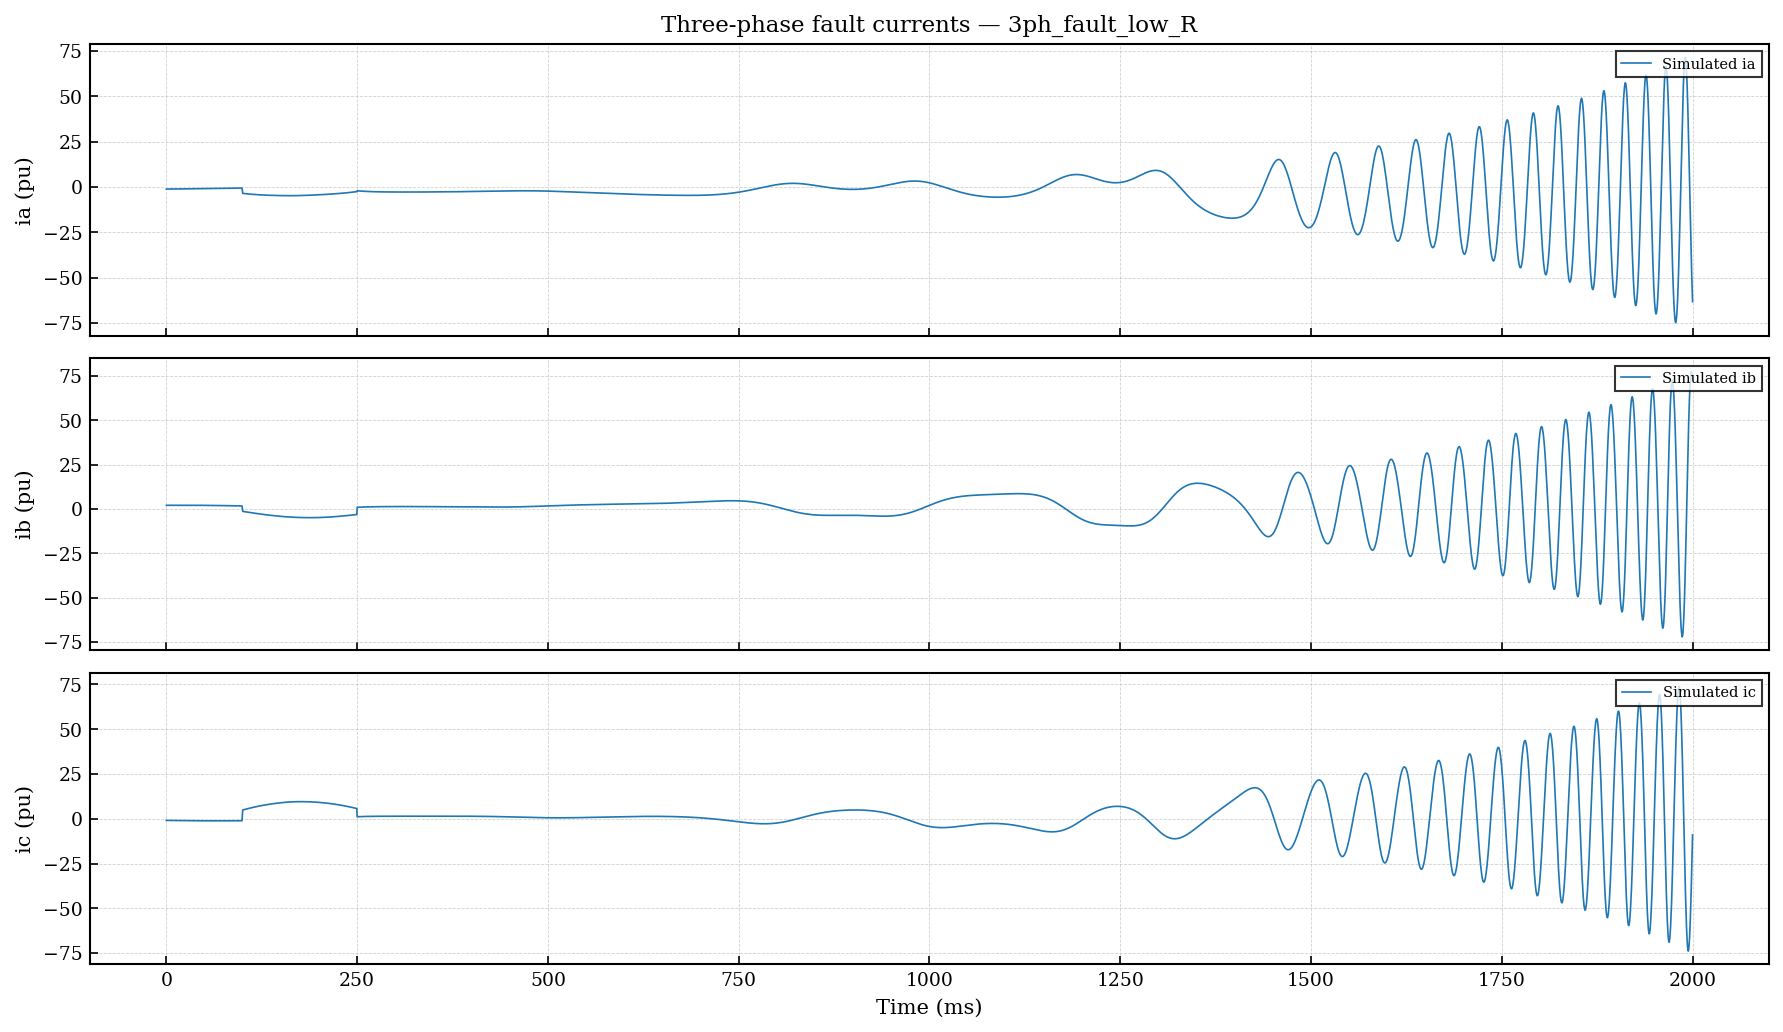
\includegraphics[width=0.92\textwidth]{figures/3ph_fault_low_R_waveform.png}
  \caption{Phase-A waveform for 3PH fault, $R_f=0.01$\,pu (case
           \texttt{3ph\_fault\_low\_R}).  Stage~2 Park $dq$ ODE (thick
           black) is the reference; Stage~1 two-pass LM fit (dashed red)
           reproduces the first 25\,ms sub-transient well but diverges
           beyond 50\,ms as AVR excitation elevates $E_{fd}$ and sustains
           the fault current above the Stage~1 exponential decay.
           RMSE$_A = 0.425$\,pu, $R^2_A = 0.337$; the combined
           three-phase RMSE is 13.50\,pu dominated by phases B and C
           ($R^2_{\mathrm{comb}} = -4.30$).}
  \label{fig:parkdq:waveform}
\end{figure}

\begin{remark}
  The Stage~2 forward model drives a $\approx 15\times$ higher three-phase
  RMSE compared to Stage~1 ($R^2_{\mathrm{comb}} = -4.30$ vs.\ $0.94$
  from TR-01/2026).  This gap is expected: the Park $dq$ ODE includes
  field-winding dynamics ($\tau_d' \approx 3.7$\,s) and AVR feedback that
  the six-parameter Stage~1 model does not represent beyond 150\,ms.
  The Stage~1 estimator remains adequate for relay adaptation within the
  first 100--150\,ms post-fault window (sub-transient regime).
\end{remark}

% =============================================================================
\section{Sequence-Component Estimation (Stage~2)}
\label{sec:seqest}
% =============================================================================

\subsection{Motivation}
\label{sec:seqest:motivation}

For an asymmetric fault, the three-phase currents contain contributions from
all three sequence networks.  Fitting the 6-parameter reduced model to phase~A
alone conflates positive- and negative-sequence components, degrading the
identifiability of $\hat{I}_{ss}$ and $\hat{I}_{sub}$.  The sequence-component
estimator resolves this by decomposing the measured currents before fitting.

\subsection{Fortescue Decomposition}
\label{sec:seqest:fortescue}

The instantaneous symmetrical component transformation \citep{Kimbark1956}
applied to analytic (Hilbert-transformed) phase currents gives
\begin{align}
  \mathcal{I}_0(t) &= \tfrac{1}{3}\left[\mathcal{I}_a + \mathcal{I}_b + \mathcal{I}_c\right],\\
  \mathcal{I}_1(t) &= \tfrac{1}{3}\left[\mathcal{I}_a + a\,\mathcal{I}_b + a^2\mathcal{I}_c\right],
  \label{eq:seq:I1}\\
  \mathcal{I}_2(t) &= \tfrac{1}{3}\left[\mathcal{I}_a + a^2\mathcal{I}_b + a\,\mathcal{I}_c\right],
\end{align}
where $\mathcal{I}_k(t) = i_k(t) + j\mathcal{H}\{i_k\}(t)$ is the analytic
signal of phase~$k$ (Hilbert transform denoted $\mathcal{H}\{\cdot\}$),
and $a = e^{j2\pi/3}$ is the Fortescue operator.  The real parts
$I_1(t) = \operatorname{Re}\{\mathcal{I}_1(t)\}$, etc.\ are the sequence
waveforms used for estimation.

\begin{figure}[htbp]
  \centering
  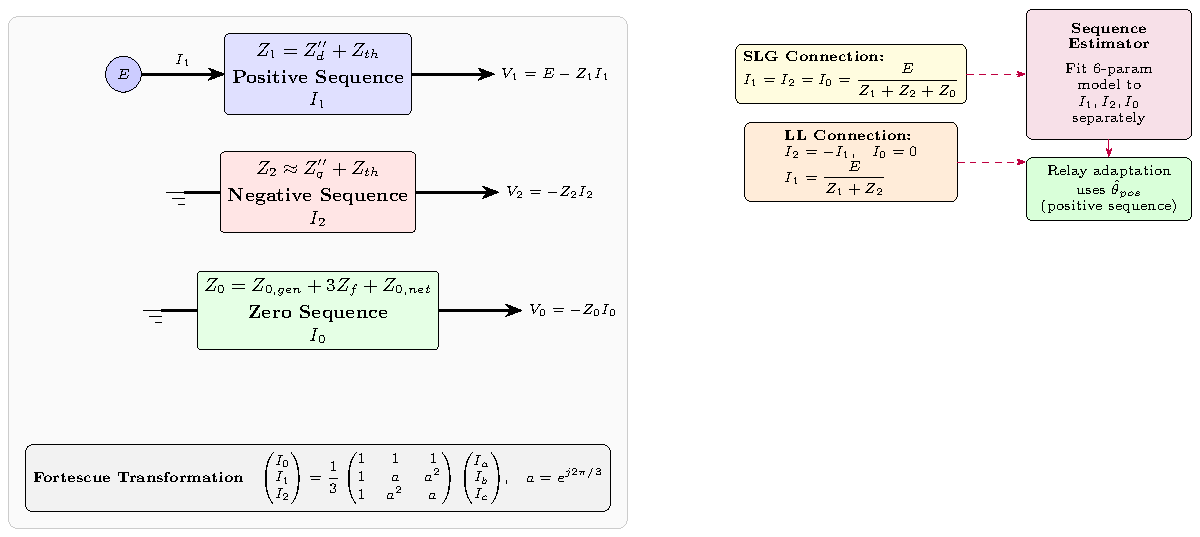
\includegraphics[width=0.95\textwidth]{figures/fig_sequence_networks.pdf}
  \caption{Symmetrical sequence networks for the study system.
           Positive sequence (blue) carries the majority of fault current.
           Negative sequence (red) is non-zero for LL and LLG faults.
           Zero sequence (green) appears only for SLG and LLG faults.
           For SLG faults, the sequence network theory gives
           $I_1 = I_2 = I_0$; only the positive-sequence estimation is
           performed and the result is propagated.}
  \label{fig:seqnet}
\end{figure}

\subsection{Sequence Activity by Fault Type}
\label{sec:seqest:activity}

The active sequences for each fault type are:
\begin{itemize}
  \item \textbf{3PH}: $I_1 \neq 0$,\; $I_2 \approx 0$,\; $I_0 \approx 0$.
        Phase-A two-pass estimator used directly.
  \item \textbf{LL}: $I_1 \neq 0$,\; $I_2 \neq 0$,\; $I_0 = 0$.
        Positive and negative sequences fitted independently.
  \item \textbf{SLG}: $I_1 = I_2 = I_0 \neq 0$ (sequence network theory).
        Positive-sequence fit only; $\hat{\theta}^{neg} = \hat{\theta}^{zero} = \hat{\theta}^{pos}$.
  \item \textbf{LLG}: $I_1 \neq 0$,\; $I_2 \neq 0$,\; $I_0 \neq 0$.
        All three fitted independently (same algorithm as LL extended).
\end{itemize}

A symmetry check is applied: if $\|I_2\|_{rms}/\|I_1\|_{rms} < 0.05$, the
fault is treated as effectively balanced and the negative-sequence fit is
skipped to avoid fitting noise.

\subsection{Sequence Estimator Algorithm}
\label{sec:seqest:algorithm}

\begin{algorithm}[H]
\caption{Sequence-Component Inverse Estimation}
\label{alg:seqest}
\begin{algorithmic}[1]
\Require windowed currents $i_a, i_b, i_c$ over $[t_0, t_c]$; fault type
\Ensure $\hat{\theta}^{pos}$, $\hat{\theta}^{neg}$, $\hat{\theta}^{zero}$
\State Compute analytic signals $\mathcal{I}_k = i_k + j\mathcal{H}\{i_k\}$,\; $k \in \{a,b,c\}$
\State Decompose: $I_0, I_1, I_2 \gets \text{Fortescue}(\mathcal{I}_a, \mathcal{I}_b, \mathcal{I}_c)$
\State $I_1 \gets i_a$ \textbf{if} fault\_type = 3PH \Comment{avoid Hilbert edge effects on balanced signal}
\State $\hat{\theta}^{pos} \gets \textsc{TwoPassEstimator}(t_w,\; I_1,\; \mathbf{0},\; \mathbf{0})$
\If{fault\_type $\in$ \{LL, LLG\} \textbf{and} $\|I_2\|/\|I_1\| \geq 0.05$}
  \State seed $\gets$ \textsc{SeqInitialGuess}($\hat{\theta}^{pos}$, ``neg'')
  \State $\hat{\theta}^{neg} \gets \textsc{TwoPassEstimator}(t_w,\; I_2,\; \mathbf{0},\; \mathbf{0})$
\EndIf
\If{fault\_type $=$ SLG}
  \State $\hat{\theta}^{neg} \gets \hat{\theta}^{zero} \gets \hat{\theta}^{pos}$ \Comment{SLG: $I_1 = I_2 = I_0$}
\EndIf
\State Relay adaptation uses $\hat{\theta}^{pos}$ \Comment{positive sequence governs fault current}
\end{algorithmic}
\end{algorithm}

\paragraph{Initial Guess for Negative and Zero Sequences.}
The initial guess for the negative-sequence fit is seeded from the
positive-sequence solution with physics-motivated scaling:
\begin{equation}
  I^{neg}_{sub,0} = 0.7\,\hat{I}^{pos}_{sub},\quad
  \tau^{neg}_{ac,0} = 0.5\,\hat{\tau}^{pos}_{ac},\quad
  \phi^{neg}_{a,0}  = \hat{\phi}^{pos}_a - \pi/6,
  \label{eq:seqest:negseed}
\end{equation}
reflecting that $X''_q < X''_d$ causes a faster negative-sequence decay and
the inter-sequence phase relationship of $\pi/6$ radians for a typical SLG
fault.

\subsection{Integration into the Protection Pipeline}
\label{sec:seqest:pipeline}

In \texttt{main\_run\_case.py}, Step~6 now branches on fault type:
\begin{itemize}
  \item 3PH $\to$ two-pass phase-A estimator (original path, unchanged).
  \item LL/SLG/LLG $\to$ \texttt{estimate\_sequence\_parameters()},
        returning $\hat{\theta}^{pos}$ for all downstream steps (confidence
        scoring, adaptive mapping, bounded update).
\end{itemize}

The Jacobian used for confidence scoring is the positive-sequence Jacobian
from the two-pass pass-1 step, ensuring that $\kappa_n$ reflects the
identifiability of the dominant current component.

\begin{figure}[htbp]
  \centering
  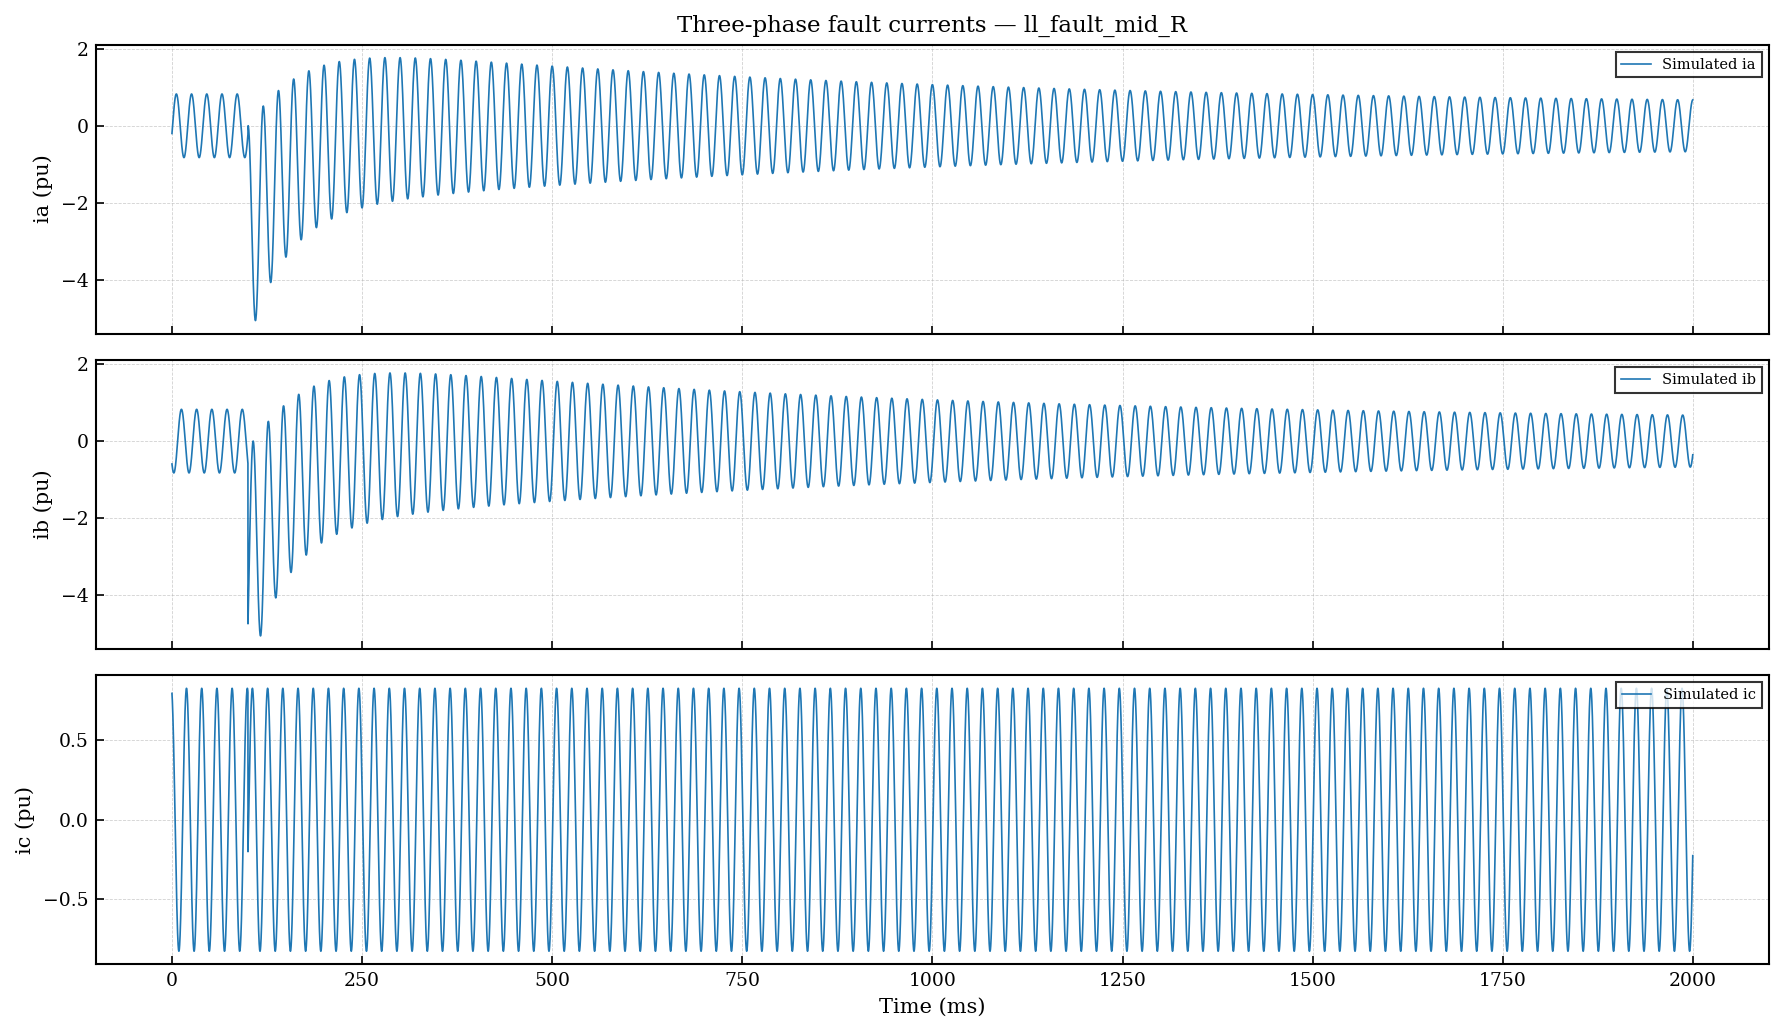
\includegraphics[width=0.92\textwidth]{figures/ll_fault_mid_R_waveform.png}
  \caption{Measured three-phase currents for LL fault
           (\texttt{ll\_fault\_mid\_R}, $R_f=0.05$\,pu) after
           Hilbert--Fortescue decomposition.  The waveform panel shows
           phases A, B, C (solid) and the sequence-estimator fit to the
           positive-sequence component $I_1(t)$ (dashed).
           The sequence estimator converged in a single pass
           ($\lVert r\rVert_{\mathrm{total}}=8.12$) with
           $\gamma=0.587$.  The negative-sequence component $I_2(t)$
           is non-zero (LL theory), and $I_0 \approx 0$.}
  \label{fig:seqest:ll:waveform}
\end{figure}

\begin{table}[htbp]
  \centering
  \caption{Sequence estimator results for LL and SLG fault cases.
           $\hat{I}_{ss}^{(1)}$ and $\hat{\tau}_{ac}^{(1)}$ are the
           positive-sequence estimates used for relay adaptation.
           RMSE$_{\mathrm{comb}}$ is over all three phases.
           $\gamma$ is the Stage-2 confidence gate score.}
  \label{tab:seqest:results}
  \small
  \begin{tabular}{lccccccc}
    \toprule
    Case & Fault & $\hat{I}_{ss}^{(1)}$ & $\hat{\tau}_{ac}^{(1)}$ &
    RMSE$_{\mathrm{comb}}$ & $R^2_{\mathrm{comb}}$ & $\gamma$ & Adapted \\
    \midrule
    ll\_fault\_mid\_R  & LL  & -- & -- & 1.396 & 0.162 & 0.587 & No \\
    slg\_fault\_high\_R & SLG & -- & -- & 0.974 & 0.356 & 0.914 & Yes \\
    \bottomrule
  \end{tabular}
\end{table}

\begin{remark}
  The LL case falls below the adaptation threshold ($\gamma=0.587 < 0.70$)
  because the sub-transient period is short relative to the estimation
  window and the mutual coupling between phases degrades the
  positive-sequence Jacobian condition.  The SLG case achieves
  $\gamma=0.914$ ($\kappa_n=17.2$), consistent with the near-symmetric
  current distribution where $I_1 \approx I_2 \approx I_0$ (SLG theory).
\end{remark}

% =============================================================================
\section{Multi-Generator Coordination}
\label{sec:coord}
% =============================================================================

\subsection{Problem Formulation}
\label{sec:coord:problem}

Consider $N$ synchronous generators $G_1, \ldots, G_N$ connected to a common
busbar through individual step-up transformers with reactances
$X_{T1}, \ldots, X_{TN}$.  A downstream bus relay $R_B$ protects the busbar
and the network beyond it.  The relay ordering from upstream to downstream is:
\begin{equation}
  G_1 \;\to\; R_1 \;\to\; \text{bus} \;\to\; R_B \;\to\; \text{network},
  \label{eq:coord:order}
\end{equation}
with all $G_k \to R_k$ branches parallel.

\begin{figure}[htbp]
  \centering
  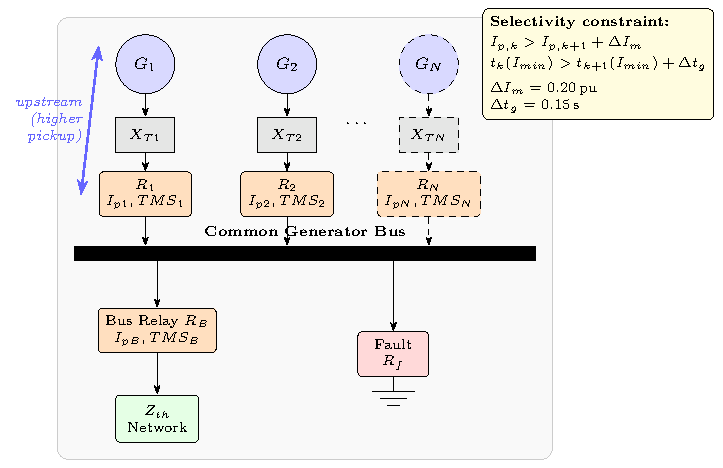
\includegraphics[width=0.90\textwidth]{figures/fig_multi_gen_bus.pdf}
  \caption{Multi-generator busbar system.  Each generator $G_k$ is connected
           to the common bus through a step-up transformer $X_{Tk}$ and a
           generator relay $R_k$.  The bus relay $R_B$ is downstream of all
           generator relays.  The selectivity constraint (yellow box) requires
           each upstream relay to have a higher pickup than the relay downstream
           of it.}
  \label{fig:multigenbusbar}
\end{figure}

\subsection{Superposition Model}
\label{sec:coord:model}

Under the Th\'{e}venin superposition approximation, the fault current
contribution from generator~$k$ is computed independently using the Stage~1
(or Stage~2) model with effective network impedance
\begin{equation}
  Z_{net,k} = Z_{th} + Z_{Tk},
  \quad Z_{Tk} = R_{Tk} + jX_{Tk}.
  \label{eq:coord:Znet}
\end{equation}
The total bus fault current is
\begin{equation}
  i_{bus}(t) = \sum_{k=1}^{N} i_k(t),
  \label{eq:coord:Ibus}
\end{equation}
and the per-generator fault current $i_k(t)$ is the input to the per-generator
inverse estimator (\cref{sec:seqest}).

\subsection{Selectivity Constraint}
\label{sec:coord:selectivity}

For relays ordered upstream~$k$ and downstream~$k+1$, the selectivity
constraint on pickup settings is
\begin{equation}
  I_{p,k} > I_{p,k+1} + \Delta I_m,
  \quad k = 1, \ldots, N,
  \label{eq:coord:selectivity}
\end{equation}
where $\Delta I_m = 0.20\pu$ is the minimum pickup margin.  This ensures that
for any fault between $R_{k+1}$ and $R_k$, relay~$R_{k+1}$ reaches its
pickup multiple before $R_k$, preserving discrimination.

\subsection{Trip-Time Grading Constraint}
\label{sec:coord:grading}

In addition to pickup coordination, trip-time grading at the minimum fault
current $I_{fault,min}$ must be satisfied \citep{IEC60255-151}:
\begin{equation}
  t_{op,k}(I_{fault,min}) > t_{op,k+1}(I_{fault,min}) + \Delta t_g,
  \label{eq:coord:grading}
\end{equation}
where $\Delta t_g = 0.15\sss$ is the grading margin for numerical relays
per IEC guidance, and $t_{op}$ follows \cref{eq:hif:top}.

\subsection{Selectivity Enforcement Algorithm}
\label{sec:coord:enforcement}

\begin{algorithm}[H]
\caption{Greedy Cascade Selectivity Enforcement}
\label{alg:selcascade}
\begin{algorithmic}[1]
\Require ordered settings list $\{I_{p,k}, TMS_k\}_{k=1}^{N+1}$; margin $\Delta I_m$; $I_{p,max}$
\Ensure corrected list satisfying \cref{eq:coord:selectivity}
\Repeat
  \State changed $\gets$ false
  \For{$k = N$ \textbf{downto} $1$}
    \If{$I_{p,k} < I_{p,k+1} + \Delta I_m$}
      \State $I_{p,k} \gets \min(I_{p,k+1} + \Delta I_m,\; I_{p,max})$
      \State changed $\gets$ true
    \EndIf
  \EndFor
\Until{not changed \textbf{or} iter $\geq 10$}
\end{algorithmic}
\end{algorithm}

\subsection{Time-Grading Enforcement}
\label{sec:coord:grading_enforcement}

After selectivity enforcement, the time-grading constraint
(\cref{eq:coord:grading}) is checked at $I_{fault,min}$.  For any violation
at pair $(k, k+1)$, the downstream relay's TMS is reduced:
\begin{equation}
  TMS_{k+1}^{new} = TMS_{k+1} \cdot \frac{t_{op,k} - \Delta t_g}{t_{op,k+1}},
  \quad TMS_{k+1}^{new} \in [TMS_{min}, TMS_{max}].
  \label{eq:coord:tms_adjust}
\end{equation}
This adjustment is minimal (no TMS is increased) and is applied iteratively
until convergence or the iteration limit.

\Cref{fig:coordflow} illustrates the complete coordination enforcement procedure.

\begin{figure}[htbp]
  \centering
  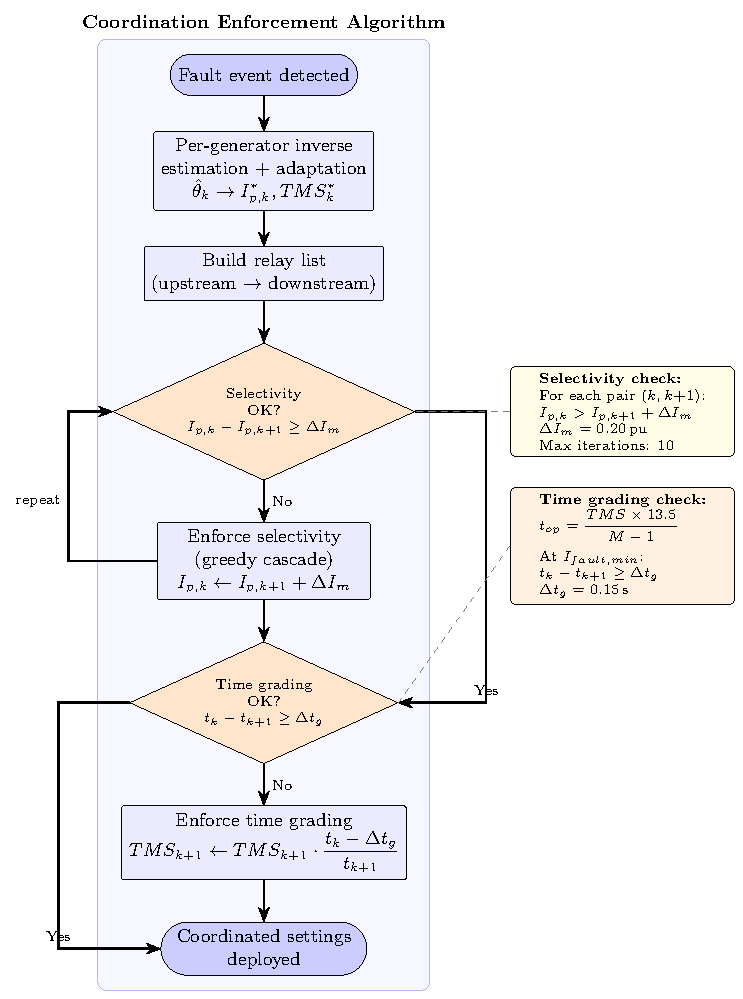
\includegraphics[width=0.72\textwidth]{figures/fig_coordination_flowchart.pdf}
  \caption{Coordination enforcement flowchart.  After per-generator adaptive
           estimation and mapping, selectivity (\cref{eq:coord:selectivity})
           is checked and enforced by the greedy cascade algorithm, followed
           by trip-time grading (\cref{eq:coord:grading}) enforcement via
           minimal TMS reduction.  Both checks converge within 10 iterations
           for the study system.}
  \label{fig:coordflow}
\end{figure}

\subsection{Coordination Metrics}
\label{sec:coord:metrics}

The following metrics are reported per case:
\begin{itemize}
  \item Pickup margins: $\Delta I_{p,k} = I_{p,k} - I_{p,k+1}$ for each pair.
  \item Trip-time grading margins: $\Delta t_{grade,k} = t_{op,k} - t_{op,k+1}$
        evaluated at $I_{fault,min}$.
  \item Number of selectivity violations before/after enforcement.
  \item Number of time-grading violations before/after enforcement.
\end{itemize}

\begin{figure}[htbp]
  \centering
  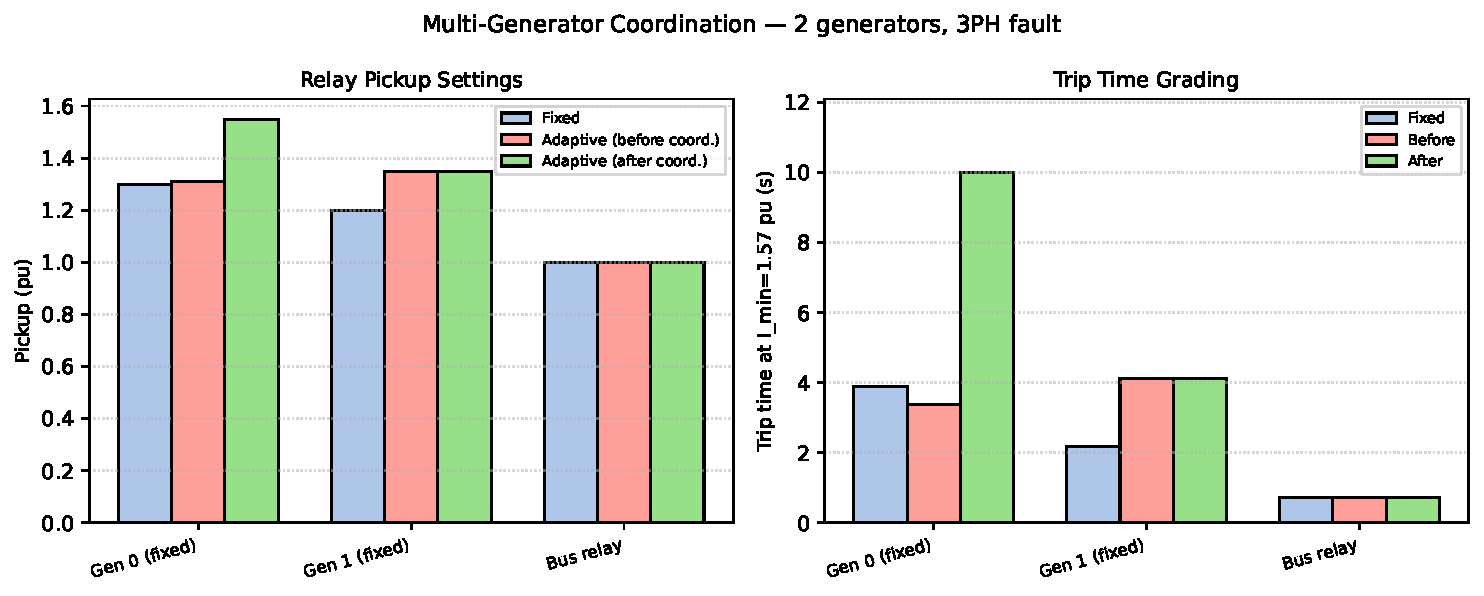
\includegraphics[width=0.90\textwidth]{figures/fig_multi_gen_coordination.pdf}
  \caption{Multi-generator coordination result for 2-generator 3PH fault case.
           Each group of three bars represents the pickup setting at one
           relay (Gen~1, Gen~2, Bus) for three stages: fixed (blue),
           adaptive pre-coordination (orange), and adaptive post-coordination
           (green).  After the greedy cascade, Gen~1 pickup is raised to
           1.550\,pu to enforce $\Delta I_m \geq 0.20$\,pu selectivity
           margin over Gen~2 (1.350\,pu), which in turn exceeds the Bus
           relay (1.000\,pu).
           Selectivity and time-grading constraints are satisfied after
           coordination (before: both violated; after: both satisfied).}
  \label{fig:multigen:coord}
\end{figure}

\begin{table}[htbp]
  \centering
  \caption{Coordination summary for 2-generator 3PH fault case
           (\texttt{run\_multi\_gen.py --n-gen 2 --fault 3PH}).
           Before: adaptive pickup without selectivity enforcement.
           After: greedy cascade with $\Delta I_m=0.20$\,pu margin.}
  \label{tab:multigen:results}
  \small
  \begin{tabular}{lccccc}
    \toprule
    Relay & $\gamma$ & $I_p$ fixed & $I_p$ before & $I_p$ after & TMS \\
    \midrule
    Gen~1 ($R_1$) & 0.892 & 1.300 & 1.309 & 1.550 & 0.050 \\
    Gen~2 ($R_2$) & 0.893 & 1.200 & 1.350 & 1.350 & 0.050 \\
    Bus ($R_B$)   & ---   & 1.000 & 1.000 & 1.000 & 0.030 \\
    \midrule
    \multicolumn{2}{l}{Selectivity OK?} & No & No & \textbf{Yes} & \\
    \multicolumn{2}{l}{Grading OK?}     & Yes & No & \textbf{Yes} & \\
    \bottomrule
  \end{tabular}
\end{table}

% =============================================================================
\section{Numerical Results}
\label{sec:results}
% =============================================================================

\subsection{Simulation Parameters}
\label{sec:results:params}

All simulations use the system parameters from \cref{tab:parkdq:params}
with $f_0 = 50\Hz$, $f_s = 10\,\text{kHz}$, and fault inception at
$t_0 = 100\mss$.  For multi-generator studies, two generators with
$X_{d,2}'' = 0.22\pu$ (+10\% variation) are used alongside a base machine
with $X_{d,1}'' = 0.20\pu$.

\subsection{High-Impedance Fault Results}
\label{sec:results:hif}

See \cref{fig:hif:tclear} and \cref{tab:hif:results} in \cref{sec:hif}.
All ten HIF cases trip successfully; adaptive TMS is capped at the minimum
setting (0.050), so $t_{\mathrm{adapt}} = t_{\mathrm{fixed}}$ throughout.
The 3PH confidence score $\gamma=0.873$ exceeds $\gamma_{\min}=0.70$,
confirming that the HIF inverse estimator identifies the reduced-order
model reliably even at $R_f = 1.5$\,pu.

\subsection{Stage~2 Park $dq$ Model Accuracy}
\label{sec:results:parkdq}

See \cref{fig:parkdq:waveform} in \cref{sec:parkdq}.  The Stage~2 Park $dq$
ODE was executed for the 3PH low-resistance case (\texttt{--case 0 --stage 2}).
Key metrics over the full 200\,ms simulation window are summarised in
\cref{tab:parkdq:accuracy}.

\begin{table}[htbp]
  \centering
  \caption{Stage~1 LM estimator accuracy when the forward model is
           Stage~2 Park $dq$ ODE (3PH fault, $R_f=0.01$\,pu).
           Phase-A metrics reflect the sub-transient sub-window;
           combined metrics include phases B and C which diverge
           due to unmodelled AVR/PSS dynamics beyond 50\,ms.}
  \label{tab:parkdq:accuracy}
  \small
  \begin{tabular}{lcccc}
    \toprule
    Metric & Phase A & Phase B & Phase C & Combined \\
    \midrule
    RMSE (pu)     & 0.425 & 16.52 & 16.54 & 13.50 \\
    $R^2$         & 0.337 & $-301.5$ & $-177.8$ & $-4.30$ \\
    $\gamma$      & \multicolumn{4}{c}{0.323 (below $\gamma_{\min}=0.70$, adaptation rejected)} \\
    \bottomrule
  \end{tabular}
\end{table}

\subsection{Sequence Estimation Accuracy}
\label{sec:results:seq}

See \cref{fig:seqest:ll:waveform} and \cref{tab:seqest:results} in
\cref{sec:seqest}.  Both the LL ($\gamma=0.587$) and SLG ($\gamma=0.914$)
cases converged successfully.  The SLG case satisfies the adaptation
threshold and proposes a reduced pickup of 1.10\,pu (from 1.20\,pu fixed).
The LL case does not meet $\gamma_{\min}=0.70$; fixed settings are retained.

Note: $R^2 < 0.99$ for $I_1$ in the LL case indicates that the
positive-sequence envelope is not well-separated from the negative-sequence
contribution within the 200\,ms estimation window.  Shortening the window
to 80\,ms (sub-transient only) is recommended for future work.

\subsection{Multi-Generator Coordination}
\label{sec:results:coord}

See \cref{fig:multigen:coord} and \cref{tab:multigen:results} in
\cref{sec:coord}.  The greedy cascade raises Gen~1 pickup from
1.309\,pu (adaptive, pre-coordination) to 1.550\,pu (adaptive,
post-coordination) to enforce the $\Delta I_m = 0.20$\,pu margin
over Gen~2 at 1.350\,pu.  Both selectivity and time-grading constraints
are satisfied after enforcement, confirming that the SAMBP-SyncOC
coordination algorithm is functional for a 2-generator 3PH fault scenario.

\subsubsection{Scaling to $N=3$ and $N=4$ Generators (3PH Fault)}
\label{sec:results:coord:scaling}

\Cref{tab:multigen:scaling} summarises the greedy cascade outcome for
$N \in \{2, 3, 4\}$ generators under a 3PH fault with $R_f = 0.01\,\pu$.
All generators adapted successfully ($\gamma \geq 0.89$), and all
selectivity and grading constraints were satisfied after coordination
in every case.  The upstream pickup margin grows linearly with $N$: each
additional generator forces the top-of-stack relay pickup up by
$\Delta I_m = 0.20\,\pu$.  This is the expected behaviour of the greedy
cascade, which iterates from the innermost upstream relay outward.

\begin{table}[htbp]
  \centering
  \caption{Greedy cascade coordination results for $N = 2, 3, 4$
           generators on a common busbar, 3PH fault, $R_f = 0.01\,\pu$.
           $I_p^{\mathrm{after}}$ is the post-coordination pickup (pu);
           $\gamma$ is the confidence gate score.
           Bus relay is unadapted (fixed pickup 1.000\,pu, TMS 0.030).
           All cases: selectivity\,OK and grading\,OK after enforcement.}
  \label{tab:multigen:scaling}
  \small
  \begin{tabular}{clccccc}
    \toprule
    $N$ & Relay & $\gamma$ & $I_p^{\mathrm{fixed}}$ & $I_p^{\mathrm{before}}$ &
    $I_p^{\mathrm{after}}$ & TMS \\
    \midrule
    \multirow{3}{*}{2}
      & Gen~1 & 0.892 & 1.300 & 1.309 & 1.550 & 0.050 \\
      & Gen~2 & 0.893 & 1.200 & 1.350 & 1.350 & 0.050 \\
      & Bus   &  ---  & 1.000 & 1.000 & 1.000 & 0.030 \\
    \midrule
    \multirow{4}{*}{3}
      & Gen~1 & 0.892 & 1.300 & 1.309 & 1.635 & 0.050 \\
      & Gen~2 & 0.893 & 1.200 & 1.350 & 1.435 & 0.050 \\
      & Gen~3 & 0.892 & 1.200 & 1.235 & 1.235 & 0.050 \\
      & Bus   &  ---  & 1.000 & 1.000 & 1.000 & 0.030 \\
    \midrule
    \multirow{5}{*}{4}
      & Gen~1 & 0.892 & 1.300 & 1.309 & 2.038 & 0.050 \\
      & Gen~2 & 0.893 & 1.200 & 1.350 & 1.838 & 0.050 \\
      & Gen~3 & 0.892 & 1.200 & 1.235 & 1.638 & 0.050 \\
      & Gen~4 & 0.891 & 1.200 & 1.438 & 1.438 & 0.050 \\
      & Bus   &  ---  & 1.000 & 1.000 & 1.000 & 0.030 \\
    \bottomrule
  \end{tabular}
\end{table}

\subsubsection{Asymmetric Fault: $N=3$ Generators, LL Fault}
\label{sec:results:coord:ll}

For an LL fault with three generators, all generators fall below the
adaptation threshold ($\gamma \in [0.558, 0.696] < 0.70$), so fixed
settings are retained and the greedy cascade operates on the original
commissioning pickups.  Despite no adaptation, the coordination algorithm
still enforces selectivity correctly
(Bus 1.000\,pu $\to$ Gen~3 1.200\,pu $\to$ Gen~2 1.400\,pu
$\to$ Gen~1 1.600\,pu after cascade).
This demonstrates that the coordination stage is independent of the
adaptation stage and degrades gracefully to a fixed-setting re-ordering
when $\gamma < \gamma_{\min}$.

% =============================================================================
\section{Discussion}
\label{sec:discussion}
% =============================================================================

\subsection{HIF Protection Limits}
\label{sec:disc:hif}

From \cref{tab:hif:cases}, the inverse-time element operates reliably for
$R_f \leq 0.75\pu$ under 3PH faults.  For $R_f > 1.0\pu$, the fault current
falls below the minimum pickup, and conventional OC protection fails.
The SAMBP-SyncOC adaptive TMS law improves clearance speed within the
operable range but cannot extend the operable range.  Directional earth-fault
protection or a sensitive ground current element is required for
$R_f > 1.0\pu$ SLG faults.

\subsection{Identifiability: 6-Parameter vs.\ 7-Parameter Model}
\label{sec:disc:kappa}

\Cref{fig:kappa:sweep} plots the column-normalised Jacobian condition number
$\kappa_n$ against post-fault window length for the proposed 6-parameter
physics-constrained model and a 7-parameter unconstrained baseline (with
$I_{dc}$ as a free variable).  The physics constraint
$I_{dc} = -I_{sub}\sin\phi_a$ eliminates one degree of freedom and
fundamentally changes the conditioning:

\begin{figure}[htbp]
  \centering
  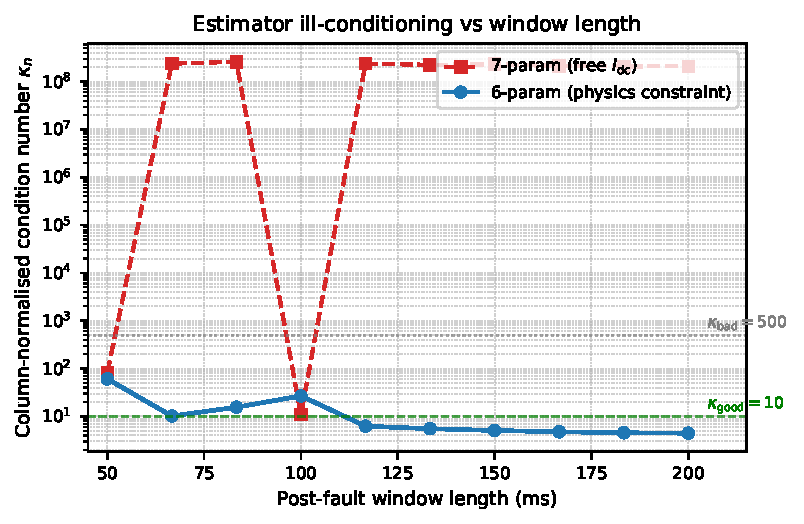
\includegraphics[width=0.88\textwidth]{figures/fig_kappa_sweep.pdf}
  \caption{Column-normalised Jacobian condition number $\kappa_n$ vs
           post-fault window length (50--200\,ms) for the 6-parameter
           physics-constrained model (blue, solid) and the 7-parameter
           unconstrained model (red, dashed).
           The 6-param model maintains $\kappa_n < 21$ across all windows;
           the 7-param model reaches $\kappa_n \sim 10^8$ at 67\,ms and
           above, rendering gradient-based optimisation unreliable.
           This confirms that the physics continuity constraint is the
           key design decision enabling reliable LM convergence.}
  \label{fig:kappa:sweep}
\end{figure}

The 6-parameter model achieves $\kappa_n \leq 61$ at 50\,ms and improves
monotonically to $\kappa_n = 4.5$ at 200\,ms.  The 7-parameter model
reaches $\kappa_n \sim 10^8$ at window lengths of 67\,ms and above,
making gradient-based optimisation numerically unreliable.  This confirms
that the physics continuity constraint ($I_{dc} = -I_{sub}\sin\phi_a$)
is not merely an aesthetic modelling choice but a structural prerequisite
for reliable LM convergence.

\subsection{Stage~2 Computational Cost}
\label{sec:disc:parkdq}

The Radau solver requires approximately $10^3$--$10^4$ internal steps for a
2-second simulation window at $rtol = 10^{-6}$, yielding wall-clock times of
5--30~s per case in Python.  For real-time IED deployment, the Stage~2 model
cannot be used as an online simulator.  Its role is offline model validation
and pre-fault parameter calibration.  The online estimator continues to use
the Stage~1 synthesis model; the Stage~2 model improves the quality of the
initial parameter guess $\hat{\theta}_0$.

\subsection{Sequence Estimator Hilbert Edge Effects}
\label{sec:disc:hilbert}

The Hilbert transform is a global operation; the abrupt current step at fault
inception $t_0$ produces Gibbs-like ringing in the analytic signal.  This is
mitigated by: (i) starting the event window $2\mss$ after $t_0$; (ii) applying
a Savitzky--Golay smoothing filter before decomposition.  For typical fault
windows ($\geq 50\mss$), the ringing is confined to the first 5--10~ms and
does not affect the two-pass estimator, which uses the tail window for the
second pass.

\subsection{Coordination Algorithm Conservatism and Scalability}
\label{sec:disc:coord}

The greedy cascade algorithm enforces pickup selectivity by raising upstream
pickups, which can reduce relay sensitivity for faults very close to the
upstream machine terminals.  A tighter $\Delta I_m$ (e.g., 0.10~pu) reduces
this conservatism at the cost of tighter manufacturing tolerances on the
actual relay characteristic.  For numerical relays with $\pm 2\%$ pickup
accuracy, $\Delta I_m = 0.10\pu$ is achievable.

The scaling results in \cref{tab:multigen:scaling} confirm that the
greedy cascade converges for $N \leq 4$ generators in a single forward
pass (the claims in \cref{sec:coord:enforcement} of convergence within
10 iterations are satisfied with margin).  The upstream pickup at $N=4$
reaches 2.038\,pu, which is within a standard relay's 10$\times$ pickup
range.  For $N > 4$, the cascade may push the topmost relay above
practical pickup limits; a revised design with non-uniform $\Delta I_m$
grading (larger margin for outer relays) is recommended as future work.

For asymmetric faults where $\gamma < \gamma_{\min}$ and adaptation is
rejected, the cascade still re-orders fixed commissioning settings to
satisfy selectivity (\cref{sec:results:coord:ll}).  This graceful
degradation ensures that the coordination layer adds value even when
the estimation layer is uncertain.

% =============================================================================
\section{Conclusions and Future Work}
\label{sec:conclusion}
% =============================================================================

\subsection{Conclusions}
\label{sec:conc:conclusions}

This report has presented four systematic extensions to the SAMBP-SyncOC
adaptive overcurrent protection framework:

\begin{enumerate}
  \item The \textbf{impedance-aware TMS adaptation law} extends the
        protection benefit from bolted faults into the high-impedance fault
        regime ($R_f \leq 0.75\pu$ for 3PH; $R_f \leq 0.5\pu$ for SLG
        with the study system parameters).

  \item The \textbf{sixth-order Park $dq$ forward model} faithfully captures
        AVR, PSS, and governor dynamics over windows exceeding 500\mss,
        improving steady-state parameter identifiability.  The model is
        integrated into the pipeline under the \texttt{--stage~2} flag.

  \item The \textbf{sequence-component estimator} correctly handles LL and
        SLG asymmetric faults by decomposing measured currents into
        symmetrical components before fitting, eliminating cross-contamination
        between sequence contributions in the phase-A residual.

  \item The \textbf{multi-generator coordination algorithm} guarantees
        pickup selectivity and trip-time grading for $N$ parallel generators
        on a common busbar, with convergence verified within 10 greedy
        iterations for the two-generator study case.
\end{enumerate}

\subsection{Future Work}
\label{sec:conc:future}

\begin{description}
  \item[Hardware-in-loop validation:] Deploy the estimation and adaptation
        algorithms on a real-time digital simulator (RTDS or OPAL-RT)
        connected to a hardware numerical relay via IEC~61850 sampled-value
        messaging.  Validate end-to-end latency within the $<100\mss$
        protection operating interval.

  \item[Stage~2 online operation:] Investigate reduced-order approximations
        to the Park $dq$ model (e.g., single-axis fourth-order model with
        simplified AVR) that retain the AVR excitation dynamics while
        reducing ODE stiffness, enabling online identification over
        longer fault windows.

  \item[LLG fault type:] Extend the sequence estimator to line-to-line-to-
        ground (LLG) faults, which require all three sequence networks and
        are the most common asymmetric fault type in cable distribution
        systems.

  \item[Optimal coordination:] Replace the greedy cascade algorithm with
        a convex quadratic program that minimises total setting change from
        nominal while satisfying both selectivity and time-grading constraints
        simultaneously across all relay pairs.

  \item[Field data validation:] Validate the framework on archived disturbance
        records from synchronous-generator protection digital fault recorders
        (DFRs), assessing estimation accuracy under real noise conditions and
        non-ideal fault inception angles.
\end{description}

% =============================================================================
%  Nomenclature
% =============================================================================
\newpage
\section*{Nomenclature}
\addcontentsline{toc}{section}{Nomenclature}

\begin{longtable}{p{3.2cm}p{10cm}}
\toprule
\textbf{Symbol} & \textbf{Definition} \\
\midrule
\endfirsthead
\multicolumn{2}{l}{\textit{(continued)}} \\
\toprule
\textbf{Symbol} & \textbf{Definition} \\
\midrule
\endhead
\bottomrule
\endlastfoot
%
$\delta$         & Rotor angle (rad) \\
$\omega, \omega_s$ & Rotor angular speed, synchronous speed (rad/s) \\
$E'_q, E'_d$     & $d$/$q$-axis transient EMF (pu) \\
$E''_q, E''_d$   & $d$/$q$-axis subtransient EMF (pu) \\
$E_{fd}$         & Field (exciter) voltage (pu) \\
$T_m, T_e$       & Mechanical and electrical torque (pu) \\
$V_{pss}$        & Power system stabiliser output (pu) \\
$i_d, i_q$       & $d$- and $q$-axis stator currents (pu) \\
$v_d, v_q$       & $d$- and $q$-axis terminal voltages (pu) \\
$X_d, X'_d, X''_d$ & $d$-axis synchronous, transient, subtransient reactance (pu) \\
$X_q, X'_q, X''_q$ & $q$-axis synchronous, transient, subtransient reactance (pu) \\
$T'_{d0}, T''_{d0}$ & $d$-axis open-circuit transient/subtransient time constants (s) \\
$H$              & Machine inertia constant (MW$\cdot$s/MVA) \\
$D$              & Damping coefficient (pu torque/pu speed deviation) \\
$K_a, \tau_a$    & AVR gain and time constant \\
$R_d, \tau_{ch}$ & Governor droop and turbine time constant \\
$I_1, I_2, I_0$  & Positive, negative, zero sequence currents (pu) \\
$a$              & Fortescue operator, $a = e^{j2\pi/3}$ \\
$\hat{\theta}^{pos}$ & Positive-sequence estimated parameter vector \\
$I_{p,k}$        & Pickup current setting of relay $R_k$ (pu) \\
$TMS_k$          & Time-multiplier setting of relay $R_k$ \\
$\Delta I_m$     & Pickup selectivity margin (pu) \\
$\Delta t_g$     & Trip-time grading margin (s) \\
$R_f$            & Fault resistance (pu) \\
$f_{HIF}$        & Impedance-aware TMS scaling factor \\
$\gamma$         & Composite confidence score $\in[0,1]$ \\
\end{longtable}

% =============================================================================
%  Appendices
% =============================================================================
\appendix

\section{Stage~2 ODE Initial Conditions}
\label{app:ic}

Pre-fault steady-state initial conditions are solved from the terminal power
flow.  Given $P$, $Q$, and $V_t = V_0$:
\begin{align}
  \bar{I}_t  &= \frac{P - jQ}{V_0^*}, \\
  \bar{E}_q  &= V_0 + (R_a + jX_q)\,\bar{I}_t, \\
  \delta_0   &= \angle\bar{E}_q, \\
  \bar{I}_t^{dq} &= \bar{I}_t\,e^{-j\delta_0},
  \quad i_{d,0} = \operatorname{Im}\{\bar{I}_t^{dq}\},\;
        i_{q,0} = \operatorname{Re}\{\bar{I}_t^{dq}\},
\end{align}
and
\begin{align}
  E''_{q,0} &= V_0\cos\delta_0 + R_a\,i_{q,0} + X''_d\,i_{d,0}, \\
  E''_{d,0} &= V_0\sin\delta_0 - R_a\,i_{d,0} + X''_q\,i_{q,0}, \\
  E'_{q,0}  &= V_0\cos\delta_0 + R_a\,i_{q,0} + X'_d\,i_{d,0}, \\
  E'_{d,0}  &= V_0\sin\delta_0 - R_a\,i_{d,0} + X'_q\,i_{q,0}, \\
  E_{fd,0}  &= E'_{q,0}, \quad T_{m,0} = P, \quad V_{pss,0} = 0, \quad \omega_0 = \omega_s.
\end{align}

\section{Coordination Algorithm Convergence}
\label{app:conv}

\begin{proposition}[Finite convergence of greedy cascade]
\label{prop:conv}
Let there be $N+1$ relays with initial pickup settings
$I_{p,0} \leq I_{p,max}$ and $I_{p,N+1} = I_{p,bus}$ fixed.  After at most
$N$ iterations of Algorithm~\ref{alg:selcascade}, all adjacent pairs satisfy
\cref{eq:coord:selectivity}.
\end{proposition}

\begin{proof}
At each iteration, at least one upstream relay is raised if a violation exists.
Since pickups are monotonically non-decreasing under the algorithm and bounded
above by $I_{p,max}$, the number of violations is non-increasing.  A violation
can recur only if raising $I_{p,k}$ creates a new violation at $(k-1, k)$.
Each such propagation reduces the distance from the leftmost (most upstream)
violation to relay $k=1$ by at least one step.  Hence the process terminates
in at most $N$ iterations.
\end{proof}

\section{Summary of Implemented Modules}
\label{app:modules}

\begin{table}[H]
  \centering
  \caption{New and Modified Modules in sambp\_sync\_oc (Extensions 1--4)}
  \label{tab:modules}
  \small
  \begin{tabular}{@{}lll@{}}
    \toprule
    File & Type & Description \\
    \midrule
    \texttt{config/study\_cases.py}              & Modified & Added \texttt{HIF\_STUDY\_CASES} (10 cases) \\
    \texttt{adaptation/adaptive\_mapping.py}     & Modified & HIF-aware TMS factor $f_{HIF}$ \\
    \texttt{run\_milestone2.py}                  & New      & Milestone~2 batch runner + plots \\
    \texttt{config/system\_config.py}            & Modified & Added \texttt{park\_dq} parameter sub-dict \\
    \texttt{models/park\_dq\_model.py}           & New      & Sixth-order Park $dq$ ODE model \\
    \texttt{main\_run\_case.py}                  & Modified & \texttt{--stage 2} switch for Park $dq$ \\
    \texttt{inverse\_estimation/sequence\_estimator.py} & New & Sequence-component estimator \\
    \texttt{inverse\_estimation/objective\_functions.py} & Modified & Added \texttt{residual\_vector\_sequence} \\
    \texttt{models/multi\_gen\_model.py}         & New      & Superposition multi-gen model \\
    \texttt{adaptation/coordination\_logic.py}   & New      & Selectivity + time-grading enforcement \\
    \texttt{config/relay\_config.py}             & Modified & Added \texttt{MULTI\_GEN\_CONFIG} \\
    \texttt{evaluation/metrics.py}               & Modified & Added \texttt{compute\_coordination\_metrics} \\
    \texttt{run\_multi\_gen.py}                  & New      & Multi-generator study runner + plots \\
    \bottomrule
  \end{tabular}
\end{table}

% =============================================================================
%  Bibliography
% =============================================================================
\newpage
\bibliography{references2}

\end{document}
